%!TEX program = xelatex
% 完整编译: xelatex -> biber/bibtex -> xelatex -> xelatex
\documentclass[lang=cn,a4paper]{elegantpaper}

\title作论文模板}
\author{Zhengqing ZHOU \\ Peking University \and Zhengqing ZHOU \\ PA Technology}
\institute{\href{https://pe.pku.edu.cn/}{体育教研部}}

\version{0.10}
\date{\zhtoday}
% Packages for automated tables
\usepackage{tabularx}
\usepackage{standalone}
\usepackage{pdflscape}
\usepackage{iftex, fancyhdr, hyperref, enumitem, fancyvrb, hologo, multirow, booktabs, bigstrut, tabularx, tocloft}
\usepackage{lipsum}

%批注
\usepackage{changes}

% 本文档命令
\usepackage{array}
\newcommand{\ccr}[1]{\makecell{{\color{#1}\rule{1cm}{1cm}}}}
\addbibresource[location=local]{reference.bib} % 参考文献,不要删除

\begin{document}

% Title Page
\begin{titlepage}
\clearpage\maketitle
\thispagestyle{empty}

\begin{abstract}
本文为 \href{https://github.com/ElegantLaTeX/ElegantPaper/}{ElegantPaper} 的说明文档。此模板基于 \LaTeX{} 的 article 类,专为工作论文写作而设计。设计这个模板的初衷是让作者不用关心工作论文的格式,专心写作,从而有更加舒心的写作体验。如果你有其他问题、建议或者报告 bug,可以在 \href{https://github.com/ElegantLaTeX/ElegantPaper/issues}{GitHub::ElegantPaper/issues} 留言。如果你想了解更多 Elegant\LaTeX{} 项目组设计的模板,请访问 \href{https://github.com/ElegantLaTeX/}{GitHub::ElegantLaTeX}。
\keywords{Elegant\LaTeX{},工作论文,模板}
\end{abstract}

\end{titlepage}


% Introduction引言
	\section{引言} \label{sec:introduction}
	定期参加体育活动(PA)对于维持整个生命周期的健康和福祉至关重要。大量证据显示在儿童和青少年中,身体活动可以显著改善身体健康(心肺和肌肉健康)、骨骼健康、认知结果(学业成绩和执行功能)、心理健康(抑郁症状机减少)以及肥胖症状减轻(WHO,2020),但在发展中国家,许多儿童仍旧无法得到充足的锻炼。当前,中国青少年的心理健康问题不容忽视。据估算,约7%~30%的中学生存在焦虑、抑郁等心理健康问题。数据显示......这一现象也引起中国政府高度重视,《“健康中国2030”规划纲要》提出要实施青少年体育活动促进计划,培养青少年体育爱好。

青少年缺少PA的一个重要的原因是其复杂、多样的决定因素,包括个人、家庭、学校和社会等多种环境因素会影响儿童和青少年行为(Biddle和Asare,2011年;Mitchell等人,2016年)。近30年的改革开放,中国一方面经历了快速的城市化和工业化发展,另一方面见证了时间最大规模的流动人口。城乡间大规模的人口流动为中国城市发展带来充足的人力和智力支持,同时也使得流动人口与本地居民的社会融入问题日益突出。事实上,这种社会空间的隔离也进一步导致流动儿童面临较为严重的城市融入问题。并且在心理发展、教育期望、学业表现等方面与本地儿童相比均处于明显的劣势(周皓、巫锡炜,2008;柳建坤等,2020;谢建社等,2011)。因此,分析和考察流动儿童和本地儿童的社会融合对青少年的健康发展、促进教育公平和城市社会的可持续发展具有重要的现实意义。为了改善家庭经济状况和生活质量,大量农村劳动力选择进程务工,同时子女也随父母远离家乡,成为了流动儿童。

作为青少年行为中啊哟关于流动儿童其父母影响运动参与问题,目前的研究或者直接分析影响流动儿童社会融入的现实障碍和影响因素。不可否认,这些研究对于我们理解流动儿童的社会融入问题具有重要意义,但它们大多忽视了流动儿童社会融入过程中的另一个重要问题——社会交往,更确切地说,是流动儿童与本地儿童之间的友谊问题。学校和家庭是青少年日常生活中最为重要的两个生活场域。学校不仅为青少年提供了适应未来工作和生活所必备的知识和技能,也同时为他们建立同伴关系和发展友谊提供了一个相对制度化的社会交往空间。然而,不同学校,甚至学校中不同班级之间,在群体构成、同辈互动情境等方面往往存在显著差异。因此,青少年在不同的学校和班级所面临的社会交往环境可能会完全不同,进而发展出迥异的社会交往关系(McFarland,etal.,2014)。更进一步说,这种社会交往关系还可能会因为青少年社会身份(如流动儿童和本地儿童)的差别而存在较为明显的差异。同样,作为社会化的另一个重要场所,家庭也对青少年的社会交往有重要影响。不同阶层的父母所持有的价值观念以及亲子间互动的方式都会潜移默化地影响青少年社会交往的方式和偏好(VanTubergenandSmith,2018)。,却只有少量国内学者注意到这一问题(史晓浩、王毅杰,2010;王毅杰、史晓浩,2010),而且也没有进行严谨的实证检验。

基于此,本文旨在考察同伴效应对青少年体育锻炼是否构成因果关系。基于国内范围最广的教育追踪调查数据,笔者使用工具变量方法消除了潜在的同伴效应内生性问题,发现同伴效应对初中生的体育锻炼时间具有正向显著影响。同时验证了了王富百慧等(2018)以及权小娟和卢春天(2020)的假设,即同伴支持同样会对个体锻炼时间有显著正向促进作用。进一步机制分析发现,班级运动氛围在同伴效应影响青少年体育锻炼时间路径中起中介作用,一方面同伴效应会显著正向促进班级运动氛围提升,另一方面,班级运动氛围同样提高个人运动参与。

综上所述,本文边际贡献主要体现在两个方面:首先,在理论上将青少年个体运动行为与教育学中经典的同伴效应问题进行连接,呼应Manski(1993,2000)等学者指出的内生性问题对同伴效应估计中造成的偏误影响,揭示了本领域研究“重相关,轻因果”传统而常忽略的遗漏变量问题。其次,实证方面,建立在教育追踪调查的数据优势允许我们使用基期调查时的同伴数据作为同伴效应的替代测量,同时将基期同伴父母的运动陪伴作为当期同伴效应的工具变量,获得了同伴效应的纯净估计值。最后,对同伴效应影响青少年体育锻炼行为的机制深入分析,班级运动氛围中介效应能够解释近20\%的总效应影响,该结论不仅从再次从学理层面验证了同伴效应对青少年体力活动促进的重要性,而且为从实践层面为合理引导学生参与体育锻炼提供了政策启示。

余下的部分安排如下,本文的第二节是文献回顾,第三节是研究设计,第四节是数据来源与数据描述,第五节是研究结果与分析,最后给出本文的结论和政策建议



基于上述讨论,本研究将着重检验当前中国初中教育阶段家庭背景和学校的班级情境对流动儿童和本地儿童之间跨群体交往的影响差异。具体来讲,通过分析“中国教育追踪调查”(CEPS)数据,本文试图回答以下问题:第一,家庭社会经济地位对青少年的跨群体交往的影响和群体差异;第二,班级情境,尤其是班级中的群体构成、同辈群体、外部群体对青少年的跨群体社会交往起到何种作用,以及对流动儿童和本地儿童又有何种差异虽然这些流动儿童会与父母生活一起,但让他们受父母工作、家庭环境等因素变化,对校园活动那个产生影响。家庭、学校和社会是儿童青少年进行体育运动的三个主要场域,其中家庭是个人社会化最初的场所,家庭教育是学校教育和社会教育的基础,大量研究已经证明,在早期的体育兴趣培养中,家庭相对于学校和社会的影响是最大的。家长的期望信念、价值信念与子女的教育期望会与PA呈高度正相关。家长对子女要求越高,与教师越匹配就荣促进参加PA。家长与子女的互动越多,对PA有正向作用。行为,家长行为会诱导孩子模仿。家长的社会资本越多,孩子可能会承接家长的交流能力,从而促进PA。同伴的家长特征,就会促进PA。比如同学的家长,陪同孩子参加课外体育锻炼、家长经常与孩子一起娱乐,都会促进孩子参加体育锻炼。中介方面,认可度较高的家长教养方式、家庭社会资本、家长教育程度、家庭经济条件也是显著因素。家庭体育是青少年行为养成的重要依托。父母作为家庭主要成员,对青少年体育锻炼参与度有广泛的影响。然而,青少年在行为养成时期,家庭因素影响占比逐渐增大。因此这一时期要格外注重家庭体育环境的建设和优化。

% Section文献综述
	\section{文献回顾} \label{sec:review}
	\input{./sub/review.tex}
% Section文献综述
	\section{研究设计} \label{sec:design}
	\input{./sub/design.tex}
% Section方法
    \section{数据来源与数据描述}\label{sec:data}
	\input{./sub/sample_statistics.tex}
% Section实证结果
    \section{研究结果与分析}\label{sec:results}
	\subsection{基准回归}
%
%\begin{center}
%\begin{figure}[h]
%\centering
%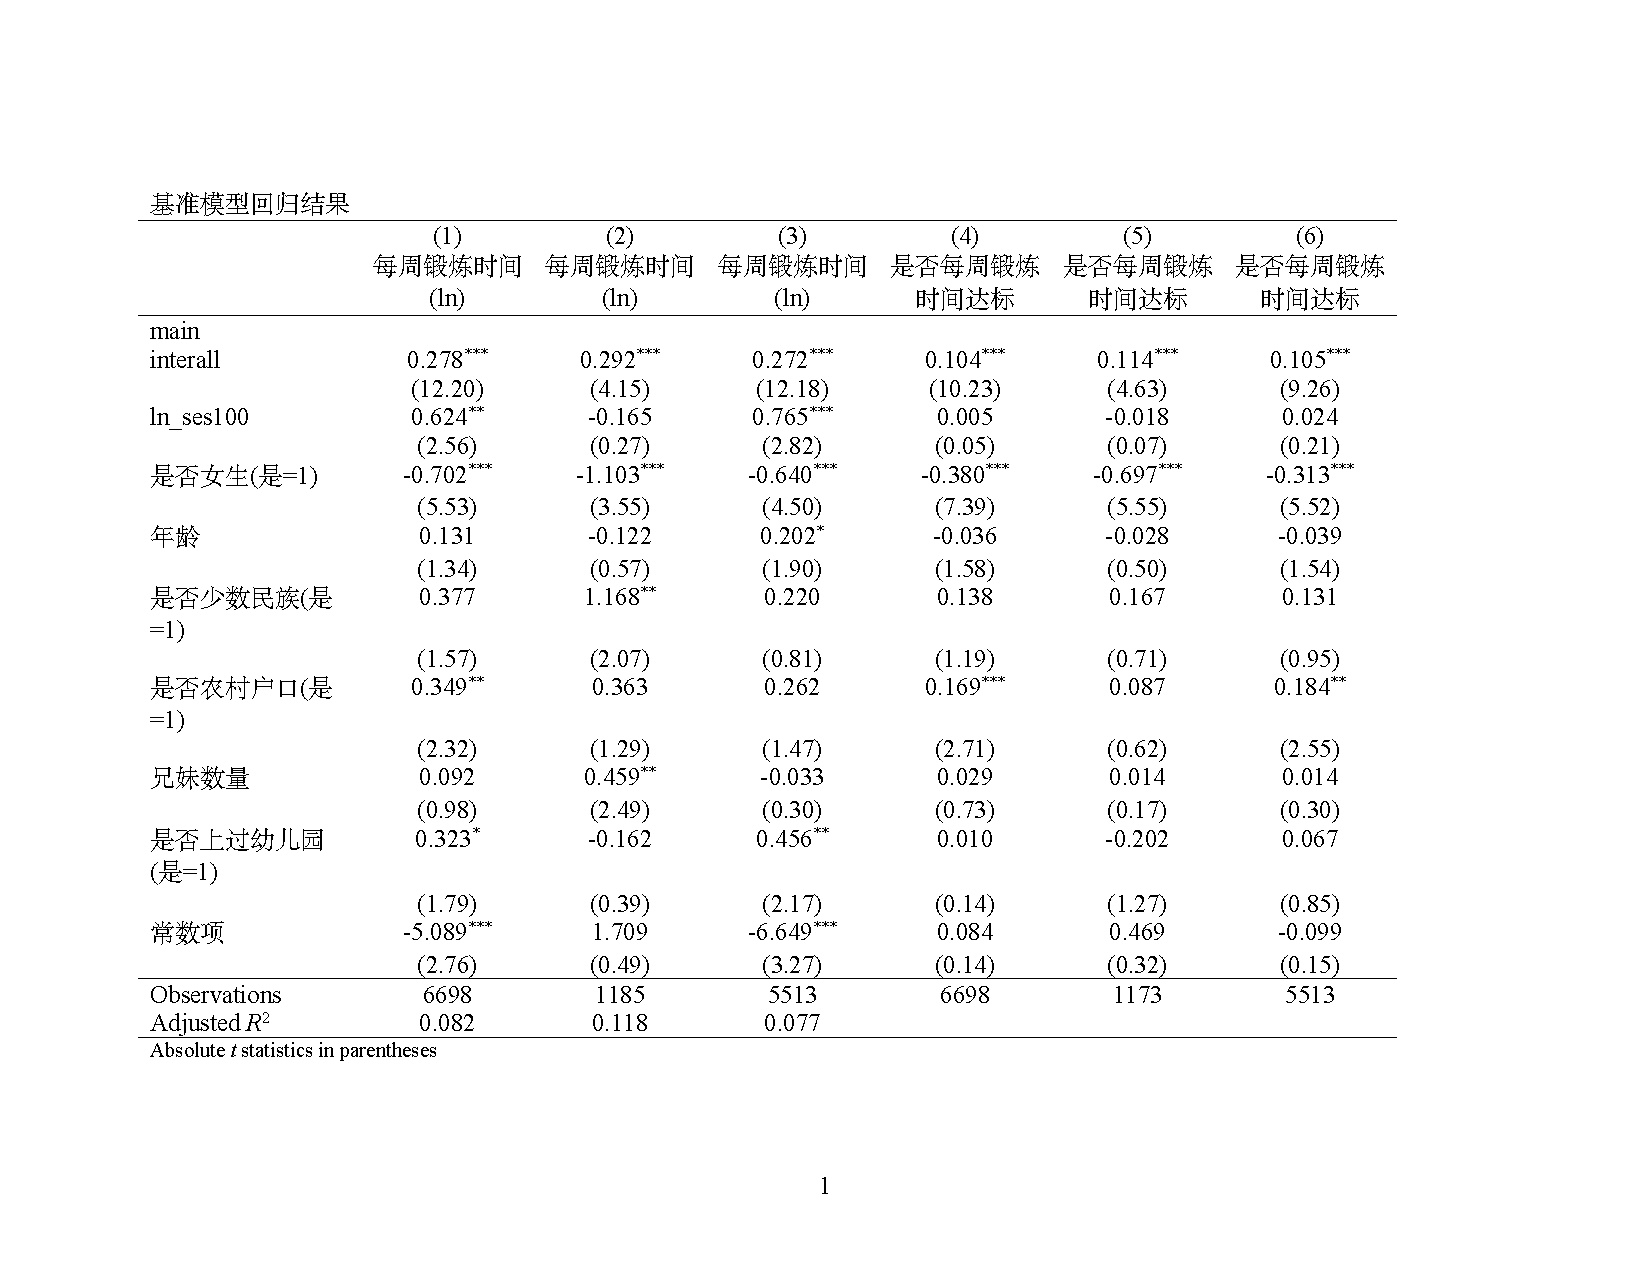
\includegraphics[width=1.25\textwidth]{figures/basigreg01.pdf}
%\caption{基准回归模型}
%\label{fig:}
%\end{figure}
%\end{center}

\subsection{异质性分析}
% Conclusion
	\section{结论} \label{sec:conclusion}
	\input{./sub/conclusion.tex}
% References
	\newpage
%	\bibliographystyle{apa}
%	\bibliography{}
	\nocite{*}
	\printbibliography[heading=bibintoc, title=\ebibname]
% Appendix
	\newpage
	\appendix
	\section{附录} \label{sec:appendix}
	
% FIGURES
\subsection{Figures}

\begin{figure}[H]
\caption{}
\centering
%\includegraphics[scale=1]{../../output/}
\label{fig:}
\end{figure}


% TABLES
\newpage
\subsection{Tables}

\begin{table}[H]
\caption{}
\centering
\begin{threeparttable}
%\input{../../output/}
\end{threeparttable}
\label{tab:}
\end{table}

	\addappheadtotoc

\end{document}